\documentclass[xelatex,ja=standard,a4paper,14pt,everyparhook=compat]{bxjsarticle}
\usepackage{amsmath, amssymb, amsthm}
\usepackage{enumerate, mleftright, mathtools}
\usepackage{caption, wrapfig}

% \usepackage{fancyhdr}
% \pagestyle{fancy}
% \fancyhead{}
% \renewcommand{\headrulewidth}{0pt}
% \fancyfoot[C]{}
% \fancyfoot[R]{\thepage}


% \usepackage{zxjatype}
% \renewcommand*\familydefault{\sfdefault}
% % なぜか Segoe UI で () が出力できない
% \setmainfont[BoldFont={Segoe UI SemiBold}]{Segoe UI}
% \setsansfont[BoldFont={Segoe UI Bold}]{Segoe UI}
% \setCJKmainfont{Noto Sans CJK JP}
% \setCJKsansfont{Noto Sans CJK JP}
% \usepackage{concmath}


\usepackage{zxjatype}
% なぜか Segoe UI で () が出力できない
% \setmainfont[BoldFont=* Bold, ItalicFont=* Italic, BoldItalicFont=* BoldItalic]{/usr/local/texlive/texmf-local/fonts/truetype/CMUConcrete/CMU Concrete.ttf}
\usepackage{concmath}
\usepackage[OT1]{fontenc}
\setsansfont{CMU Concrete}
\setmainfont{CMU Concrete}
\setCJKmainfont{Noto Sans JP}
\setCJKsansfont{Noto Sans JP}
% \newfontfamily\bfsegoe{CMU Concrete Roman}
% \renewcommand*\bfdefault{\bfsegoe}


\newcommand{\fS}{\mathfrak{S}}

\newcommand{\paren}[1]{\mleft(#1\mright)}

\theoremstyle{definition}
\newtheorem{theorem}{定理}[subsection]
\newtheorem*{theorem*}{定理}
\newtheorem{example}[theorem]{例}
\newtheorem{proposition}[theorem]{命題}
\newtheorem{corollary}[theorem]{系}
\newtheorem{fact}{Fact}
\renewcommand{\proofname}{\textup{証明}}

\begin{document}

\setcounter{section}{1}
\setcounter{subsection}{6}
\setcounter{subsubsection}{2}

\subsubsection{Min-Max Trees and the $cd$-Index}

$T(w)$($w$のCartesian tree)の変形を考える。

相異なる整数の列$w = a_1 a_2 \cdots a_n$の\textbf{min-max tree} $M(w)$を次のように定義する。
\begin{enumerate}[1.]
    \item $a_j = \min a_i$または$a_j = \max a_i$を満たす最小の$j$をとる。
    \item $a_j$を$M(w)$の根とし、左側の部分木を$M(a_1, \ldots, a_{j-1})$、右側の部分木を$M(a_{j+1}, \ldots, a_n)$とする。
\end{enumerate}
$M(w)$の頂点で、左の子だけを持つようなものは存在しないことに注意。

Min-max tree $M(w)$と$1 \leq i \leq n$について、$M(w)$の頂点の並び替え$\psi_i M(w)$を次のように定める。
\begin{enumerate}[1.]
    \item $M(w)$上で、頂点$a_i$とその右側の部分木をまとめて$M_{a_i}$とする。
    \item $a_i = \min V(M_{a_i})$の場合は、$a_i$を$\max V(M_{a_i})$に置き換え、$M_{a_i}$の残りの部分では頂点同士の大小関係を保つように並び変える。
    \item $a_i = \max V(M_{a_i})$の場合は、$a_i$を$\min V(M_{a_i})$に置き換え、残りは同様にする。
\end{enumerate}

\begin{figure}[ht]
    \centering
    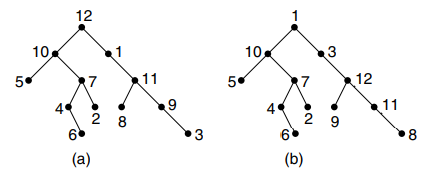
\includegraphics[width=0.7\textwidth]{1.11.png}
    \caption{(a) $M(5,10,4,6,7,2,12,1,8,11,9,3)$ \\
        (b) $\psi_7 M(\ldots)$}
\end{figure}

\begin{fact}
    $\psi_1, \ldots, \psi_n$の合成は可換であり、$\psi_i \circ \psi_i = \mathrm{id}$。ゆえにこれらは可換群$\mathfrak G_w$を生成する。$\mathfrak G_w$は$(\mathbb Z/2\mathbb Z)^{\iota(w)}$と同型(ただし$\iota(w)$は$M(w)$が持つ葉でない頂点の個数)。したがって、$\psi M(w)$ ($\psi \in \mathfrak G_w$)として得られる木は$2^{\iota(w)}$通り。
\end{fact}

$w \in \fS_n$、$\psi \in \mathfrak G_w$について、$\psi M(w) = M(\psi w)$となるように$\psi w$を定める。$v, w \in \fS_n$について、$v = \psi w$となるような$\psi \in \mathfrak G_w$が存在するとき$v$と$w$は\textbf{$M$-同値}であるといい、$v \overset{M}{\sim} w$で表す。これは同値関係。Fact 1より、$w$を含む同値類$[w]$の要素数は$2^{\iota(w)}$。

\begin{fact}
    $M(w)$の頂点$a_i$が、右の子のみを持つとする。このとき \begin{equation*}
        D(\psi_i w) = \begin{cases*}
            D(w) \cup \{i\} & if $i \notin D(w)$, \\
            D(w) - \{i\} & if $i \in D(w)$.
        \end{cases*}
    \end{equation*}
    $a_i$が左の子と右の子を持つとき、$i \in D(w)$と$i-1 \in D(w)$のちょうど片方が成立し、 \begin{equation*}
        D(\psi_i w) = \begin{cases*}
            (D(w) \cup \{i\}) - \{i-1\} & if $i \notin D(w)$, \\
            (D(w) \cup \{i-1\}) - \{i\} & if $i \in D(w)$.
        \end{cases*}
    \end{equation*}
\end{fact}

Descent set $D(w)$や木の構造の情報を、非可換な不定元$a$, $b$, $c$, $d$, $e$を用いた単項式で表すことを考える。

集合$S \subseteq [n-1]$について、その\textbf{characteristic monomial}を \begin{equation*}
    u_S = e_1 e_2 \cdots e_{n-1},
\end{equation*}
で定める。ここで \begin{equation*}
    e_i = \begin{cases*}
        a & if $i \notin S$, \\
        b & if $i \in S$,
    \end{cases*}
\end{equation*}
とする。例えば、$u_{D(37485216)} = ababbba$。

$w = a_1 a_2 \cdots a_n \in \fS_n$と$1 \leq i \leq n$について、 \begin{equation*}
    f_i = f_i(w) = \begin{cases*}
        c & if $a_i$が$M(w)$上で右の子のみを持つ, \\
        d & if $a_i$が左の子と右の子を持つ, \\
        e & if $a_i$が子を持たない,
    \end{cases*}
\end{equation*}
とする。$\Phi'_w = \Phi'_w(c,d,e) = f_1 f_2 \cdots f_n$とし、そこから$e$を削除したものを$\Phi_w = \Phi_w(c,d)$とする。例えば、$w=5,10,4,6,7,2,12,1,8,11,9,3$に対して \begin{align*}
    \Phi'_w & = edcededcedce, \\
    \Phi_w  & = dcddcdc.
\end{align*}
$\Phi_w$に対して末尾と各$d$の直前に$e$を挿入すれば$\Phi'_w$が復元できる。
$v \overset{M}{\sim} w$ならば、$\Phi'_v = \Phi'_w$と$\Phi_v = \Phi_w$が成り立つ。

\begin{fact}
    $w \in \fS_n$とし、$w$が属する$M$-同値類を$[w]$で表すとき、 \begin{equation*}
        \Phi_w(a+b, ab+ba) = \sum_{v \in [w]} u_{D(v)}.
    \end{equation*}
\end{fact}
これが成り立つことはFact 2.から確認できる。

たとえば、$w=5,10,4,6,7,2,12,1,8,11,9,3$に対して、 \begin{equation*}
    \sum_{v \in [w]} u_{D(v)} = (ab+ba)(a+b)(ab+ba)(ab+ba)(a+b)(ab+ba)(a+b).
\end{equation*}

\begin{fact}
    各同値類$[w]$は、ちょうど一つのalternating permutation(とちょうど一つのreverse alternating permutation)を含む。したがって、$w \in \fS_n$が動くときの$[w]$の種類数はオイラー数$E_n$。
\end{fact}
これはFact 3.から分かる。

ここで、母関数 \begin{align*}
    \Psi_n = \Psi_n(a, b) &= \sum_{w \in \fS_n} u_{D(w)} \\
    &= \sum_{S \in [n-1]} \beta(S) u_S,
\end{align*}
を考える。たとえば $\Psi_3 = aa + 2ab + 2ba + bb$。この多項式$\Psi_n$は$\fS_n$の\textbf{$ab$-index}と呼ばれる。

ここで \begin{equation*}
    \Psi_n = \sum_{[w]} \sum_{v \in [w]} u_{D(v)} = \sum_{[w]} \Phi_w(a+b, ab+ba),
\end{equation*}
であるから、次が成り立つ。

\begin{theorem}
    $c=a+b$、$d=ab+ba$とすると、$ab$-index $\Psi_n$は$c$、$d$の単項式$E_n$個からなる多項式として表せる。
\end{theorem}

この$c$、$d$の多項式を$\Phi_n$とし、$\fS_n$の\textbf{$cd$-index}と呼ぶ。$\Phi_n$の相異なる項の個数は、$\Phi_w$としてありうる$c$、$d$の単項式の個数、すなわちフィボナッチ数$F_n$である。

$S \subseteq [n-1]$に対して、 \begin{equation*}
    \omega(S) = \{i \in [n-2] : \text{$i \in S$と$i+1 \in S$のちょうど一方が成立する}\},
\end{equation*}
とする。

\begin{proposition}
    $S, T \subseteq [n-1]$とする。$\omega(S) \subset \omega(T)$ならば$\beta_n(S) < \beta_n(T)$。
\end{proposition}
\begin{proof}
    $w \in \fS_n$、$\Phi'_w = f_1 f_2 \cdots f_n$ ($f_i \in \{c,d,e\}$)とする。 \begin{equation*}
        S_w = \{i-1 : f_i = d\},
    \end{equation*}
    とするとき、 \begin{equation*}
        \Phi_w(a+b, ab+ba) = \sum_{v \in [w]} u_{D(v)} = \sum_{\omega(X) \supseteq S_w} u_X,
    \end{equation*}
    である。 \begin{equation*}
        \Psi_n = \sum_{S} \beta_n(S) u_s = \sum_{[w]}\sum_{v \in [w]} u_{D(v)} = \sum_{[w]} \sum_{\omega(X) \supseteq S_w} u_X
    \end{equation*}
    より、$\omega(S) \subseteq \omega(T)$ならば$\beta_n(S) \leq \beta_n(T)$。 $\omega(S) \subsetneq \omega(T)$のとき、$\omega(T) \supseteq S_w$かつ$\omega(S) \not\supseteq S_w$なる$w$が存在するので、$\beta_n(S) < \beta_n(T)$。
\end{proof}

\begin{corollary}
    $S \subseteq [n-1]$のとき、$\beta_n(S) \leq E_n$。等号成立は$S=\{1,3,5,\ldots\} \cap [n-1]$または$S=\{2,4,6,\ldots\} \cap [n-1]$のとき。
\end{corollary}

\end{document}
